% ============================================================
% IEEE Conference Paper - WebRTC Based LAN DROP for Offline File Sharing
% Compile with: pdflatex → bibtex → pdflatex × 2
% Or upload directly to Overleaf (recommended)
% ============================================================

\documentclass[conference]{IEEEtran}

% ---- Packages ----
\usepackage{cite}
\usepackage{amsmath,amssymb,amsfonts}
\usepackage{algorithmic}
\usepackage{algorithm}
\usepackage{graphicx}
\usepackage{textcomp}
\usepackage{xcolor}
\usepackage{booktabs}
\usepackage{multirow}
\usepackage{url}
\usepackage{hyperref}
\usepackage{tikz}
\usetikzlibrary{shapes.geometric, arrows.meta, positioning, fit, calc}

\hypersetup{
    colorlinks=true,
    linkcolor=black,
    citecolor=black,
    urlcolor=blue
}

\def\BibTeX{{\rm B\kern-.05em{\sc i\kern-.025em b}\kern-.08em
    T\kern-.1667em\lower.7ex\hbox{E}\kern-.125emX}}

\begin{document}

% ============================================================
% TITLE
% ============================================================
\title{WebRTC Based LAN DROP for Offline File Sharing}

% ============================================================
% AUTHORS - Replace placeholders
% ============================================================
\author{
\IEEEauthorblockN{Chetan G M}
\IEEEauthorblockA{
Department of Computer Science and Engineering\\
\textit{Gopalan College of Engineering and Management (GCEM)}\\
Bangalore, India\\
chetangm88@gmail.com}
\and
\IEEEauthorblockN{Fayaz Chittapur}
\IEEEauthorblockA{
Department of Computer Science and Engineering\\
\textit{Gopalan College of Engineering and Management (GCEM)}\\
Bangalore, India\\
fayazchittapur10@gmail.com}
}

\maketitle

% ============================================================
% ABSTRACT
% ============================================================
\begin{abstract}
Conventional file sharing approaches depend on centralized cloud servers, introducing latency, bandwidth costs, privacy concerns, and hard file-size limits. This paper presents \textbf{LAN DROP}, a WebRTC-based browser-native peer-to-peer (P2P) file transfer system designed for high-speed offline file sharing within Local Area Networks (LAN). The proposed system enables direct device-to-device file transfers without uploading data to any intermediary cloud server. A lightweight Socket.io-based signaling server facilitates automatic peer discovery by grouping clients by subnet IP, while the actual file payload traverses a direct DTLS-encrypted SCTP data channel between browsers. The system implements a chunked binary transfer pipeline with configurable chunk sizes (up to 256~KB), backpressure-aware flow control using high/low watermark thresholds, SHA-256 end-to-end integrity verification, and pause/resume capability. For scenarios where direct P2P connectivity is blocked (e.g., mobile hotspot AP isolation, symmetric NAT), the system seamlessly falls back to a WebSocket relay path, ensuring 100\% transfer completion. A Service Worker-based streaming receiver mode enables memory-efficient reception of arbitrarily large files (1~GB+). Experimental evaluation demonstrates sustained throughput exceeding 40~MB/s on gigabit LAN, sub-second peer discovery, and zero data leakage to external servers. The system is fully cross-platform, requiring no software installation---only a modern web browser.
\end{abstract}

\begin{IEEEkeywords}
WebRTC, Peer-to-Peer, File Transfer, Data Channel, SCTP, Signaling Server, Socket.io, Service Worker, Browser-Based, LAN Discovery, Backpressure Flow Control, SHA-256
\end{IEEEkeywords}

% ============================================================
% I. INTRODUCTION
% ============================================================
\section{Introduction}

File sharing remains one of the most fundamental and frequently performed operations in computing. Traditional methods---email attachments, cloud storage services (Google Drive, Dropbox, WeTransfer), and USB drives---each carry significant limitations. Email imposes strict attachment size limits (typically 25~MB). Cloud services require uploading the entire file to a remote server before the recipient can download it, doubling bandwidth consumption, introducing latency proportional to round-trip time to distant data centers, and raising privacy concerns as files transit through and are stored on third-party infrastructure~\cite{buyya2009cloud}. USB-based transfers require physical proximity and compatible hardware.

In local network environments such as offices, classrooms, and homes, devices are often on the same LAN subnet, separated by only a single switch hop. In these scenarios, routing file data through a remote cloud server is particularly wasteful---the data travels from one device to the cloud and back, even though the two devices may be mere meters apart.

WebRTC (Web Real-Time Communication)~\cite{johnston2014webrtc}, originally designed for real-time audio and video communication, includes a powerful capability: the \textbf{RTCDataChannel} API. Data channels provide a reliable, ordered, bidirectional byte stream directly between two browsers, encrypted with DTLS (Datagram Transport Layer Security)~\cite{rfc6347}, without any server intermediary. This paper leverages RTCDataChannel to build a complete, production-grade file transfer system that operates entirely within the browser.

The key contributions of this paper are:

\begin{enumerate}
    \item A \textbf{zero-configuration peer discovery} mechanism that automatically groups devices by their LAN subnet IP address, requiring no user accounts, login, or manual IP entry.
    \item A \textbf{chunked binary transfer pipeline} with serialized file-ID and sequence-index headers enabling concurrent multi-file transfers, pause/resume, and out-of-order chunk reassembly.
    \item A \textbf{backpressure-aware flow control} system using high/low watermark thresholds on the SCTP send buffer to prevent browser memory exhaustion during large file transfers.
    \item An \textbf{adaptive relay fallback} mechanism that seamlessly switches to WebSocket-based relay when direct P2P connectivity is blocked, ensuring 100\% reliability.
    \item A \textbf{Service Worker streaming receiver} that pipes incoming chunks directly to disk via the browser download manager, enabling memory-efficient transfers of arbitrarily large files.
\end{enumerate}

% ============================================================
% II. RELATED WORK
% ============================================================
\section{Related Work}

\subsection{Traditional File Transfer Protocols}
FTP (File Transfer Protocol)~\cite{rfc959} and its secure variant SFTP have been standard file transfer mechanisms for decades. However, they require dedicated server infrastructure, client software installation, and network configuration (firewall port-forwarding). HTTP-based file uploads to cloud services simplify the user experience but mandate server-side storage and double bandwidth consumption (upload + download).

\subsection{WebRTC-Based Communication}
WebRTC was standardized by the W3C and IETF to enable real-time peer-to-peer communication directly in web browsers~\cite{johnston2014webrtc}. While predominantly used for video conferencing, the RTCDataChannel API~\cite{rfc8831} enables arbitrary data transfer. Prior works such as ShareDrop~\cite{sharedrop} and Snapdrop~\cite{snapdrop} demonstrated the viability of WebRTC for file sharing but faced limitations with large files, lacked flow control mechanisms, and provided no fallback when P2P connectivity failed.

\subsection{Signaling and NAT Traversal}
WebRTC requires a signaling mechanism to exchange Session Description Protocol (SDP) offers and answers between peers. ICE (Interactive Connectivity Establishment)~\cite{rfc8445} employs STUN~\cite{rfc8489} servers to discover public IP addresses and TURN~\cite{rfc8656} servers as a relay of last resort. Our system introduces an additional, more efficient fallback: a lightweight WebSocket relay that operates over the same signaling connection, eliminating the need for dedicated TURN server infrastructure.

\subsection{Service Workers for Streaming}
The Service Worker API~\cite{w3cserviceworker} enables intercepting network requests and constructing custom responses with ReadableStream objects. This capability has been used for offline caching and progressive web apps. Our work repurposes it to stream incoming file chunks directly to the browser's download manager, bypassing in-memory buffering entirely.

% ============================================================
% III. SYSTEM ARCHITECTURE
% ============================================================
\section{System Architecture}

The proposed system follows a hybrid architecture with a thin signaling server and direct peer-to-peer data transfer. Fig.~\ref{fig:architecture} illustrates the high-level system architecture.

\begin{figure}[htbp]
\centering
\resizebox{\columnwidth}{!}{%
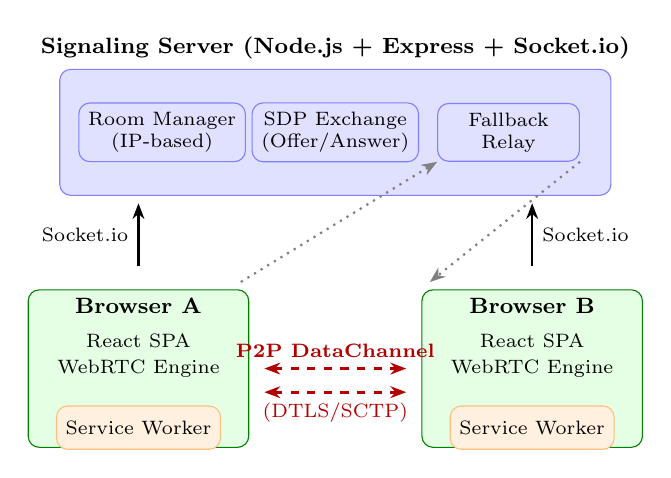
\begin{tikzpicture}[
    box/.style={draw, rounded corners=4pt, minimum width=2.2cm, minimum height=0.8cm, align=center, font=\footnotesize},
    server/.style={box, fill=blue!12, draw=blue!50},
    client/.style={box, fill=green!10, draw=green!50!black},
    worker/.style={box, fill=orange!12, draw=orange!50, minimum width=1.6cm, minimum height=0.55cm, font=\scriptsize},
    arr/.style={-{Stealth[length=2mm]}, thick},
    darr/.style={{Stealth[length=2mm]}-{Stealth[length=2mm]}, thick},
]

% Signaling Server
\node[server, minimum width=7cm, minimum height=1.6cm] (server) at (0, 3.5) {};
\node[font=\footnotesize\bfseries, above] at (server.north) {Signaling Server (Node.js + Express + Socket.io)};
\node[server, minimum width=1.8cm, minimum height=0.5cm, font=\scriptsize] (room) at (-2.2, 3.5) {Room Manager\\(IP-based)};
\node[server, minimum width=1.8cm, minimum height=0.5cm, font=\scriptsize] (sdp) at (0, 3.5) {SDP Exchange\\(Offer/Answer)};
\node[server, minimum width=1.8cm, minimum height=0.5cm, font=\scriptsize] (relay) at (2.2, 3.5) {Fallback\\Relay};

% Browser A
\node[client, minimum width=2.8cm, minimum height=2cm] (browserA) at (-2.5, 0.5) {};
\node[font=\footnotesize\bfseries] at (-2.5, 1.3) {Browser A};
\node[font=\scriptsize] at (-2.5, 0.85) {React SPA};
\node[font=\scriptsize] at (-2.5, 0.5) {WebRTC Engine};
\node[worker] (swA) at (-2.5, -0.25) {Service Worker};

% Browser B
\node[client, minimum width=2.8cm, minimum height=2cm] (browserB) at (2.5, 0.5) {};
\node[font=\footnotesize\bfseries] at (2.5, 1.3) {Browser B};
\node[font=\scriptsize] at (2.5, 0.85) {React SPA};
\node[font=\scriptsize] at (2.5, 0.5) {WebRTC Engine};
\node[worker] (swB) at (2.5, -0.25) {Service Worker};

% Arrows
\draw[arr] (-2.5, 1.8) -- (-2.5, 2.6) node[midway, left, font=\scriptsize] {Socket.io};
\draw[arr] (2.5, 1.8) -- (2.5, 2.6) node[midway, right, font=\scriptsize] {Socket.io};

% P2P Arrow
\draw[darr, color=red!70!black, dashed, very thick] (-0.9, 0.5) -- (0.9, 0.5) node[midway, above, font=\scriptsize\bfseries, color=red!70!black] {P2P DataChannel};
\draw[darr, color=red!70!black, dashed, very thick] (-0.9, 0.2) -- (0.9, 0.2) node[midway, below, font=\scriptsize, color=red!70!black] {(DTLS/SCTP)};

% Fallback path
\draw[arr, color=gray, dotted] (-1.2, 1.6) -- (relay.south west) node[midway, left, font=\tiny, color=gray] {};
\draw[arr, color=gray, dotted] (relay.south east) -- (1.2, 1.6) node[midway, right, font=\tiny, color=gray] {};

\end{tikzpicture}
}
\caption{System Architecture of LAN DROP showing dual-path connectivity: direct P2P via WebRTC DataChannel (primary) and WebSocket relay via Signaling Server (fallback).}
\label{fig:architecture}
\end{figure}

\subsection{Signaling Server}
The signaling server is implemented using Node.js with Express for static file serving and Socket.io for bidirectional real-time communication. Its responsibilities are strictly limited to:

\textbf{Room Management:} When a client connects, the server extracts its IP address from the HTTP request headers. Clients sharing the same IP subnet are grouped into the same logical ``room.'' This enables zero-configuration discovery---devices on the same LAN automatically see each other without any manual pairing.

\textbf{SDP Relay:} The server forwards WebRTC SDP Offer and Answer messages between peers. These messages contain session parameters (codecs, encryption keys, ICE candidates) but never contain file payload data.

\textbf{ICE Candidate Relay:} ICE candidates discovered by each peer's browser are relayed to the remote peer via the signaling server. The server also augments mDNS \texttt{.local} candidates with real IP addresses to improve connectivity on networks that do not support mDNS resolution.

\textbf{Fallback Message Relay:} When direct P2P connectivity fails, the server relays binary file chunks as Socket.io messages, acting as a transparent proxy.

\subsection{Client Application}
The client is a single-page application (SPA) built with React~17 and bundled using Rspack. It manages peer discovery UI (radar-style display), WebRTC connection lifecycle, file chunking pipeline, transfer state management (progress, pause/resume, speed, ETA), and QR code pairing for cross-network discovery.

\subsection{Service Worker}
A Service Worker intercepts fetch requests matching a specific URL pattern and responds with a \texttt{ReadableStream} constructed from incoming file chunks. This enables the browser's native download manager to write received data directly to disk, keeping memory consumption near zero even for multi-gigabyte transfers.

% ============================================================
% IV. METHODOLOGY
% ============================================================
\section{Methodology}

\subsection{Peer Discovery Protocol}
Upon loading the application, each client: (1) generates a unique 8-character alphanumeric device identifier stored in \texttt{sessionStorage}; (2) establishes a Socket.io WebSocket connection to the signaling server; (3) emits a \texttt{JOIN\_ROOM} event with its device ID and device type; (4) the server groups this client by its source IP address and broadcasts a \texttt{JOINED\_ROOM} event to all existing members; (5) the new client receives a \texttt{JOINED\_MEMBER} event containing the list of all current peers. This IP-based grouping ensures that devices behind the same NAT gateway are automatically placed in the same room.

\subsection{WebRTC Connection Establishment}
When a user selects a peer for file transfer, the initiating peer creates an \texttt{RTCPeerConnection} with STUN server configuration (\texttt{stun.l.google.com:19302}, \texttt{stun.cloudflare.com:3478}). A named \texttt{RTCDataChannel} (``FileTransfer'') is created with \texttt{ordered: true} and \texttt{maxRetransmits: 50} for reliable delivery. An SDP Offer is generated, exchanged via the signaling server, and upon successful ICE connectivity check, the DTLS handshake completes and the data channel opens.

\subsection{Adaptive Fallback Mechanism}
A 2.5-second watchdog timer is started when a connection attempt begins. If the \texttt{connectionState} does not reach \texttt{"connected"} within this window (common on mobile hotspots with AP isolation), the system seamlessly activates a local relay fallback mode. File chunks are sent as Socket.io \texttt{SEND\_MESSAGE} events through the signaling server. The transfer experience remains identical to the user---same progress bar, speed, and ETA.

\subsection{Binary Chunk Serialization}
Each file is divided into chunks of configurable size (bounded by \texttt{maxMessageSize}, capped at 256~KB). Each chunk is serialized with a fixed-size binary header as specified in Table~\ref{tab:chunkformat}.

\begin{table}[htbp]
\caption{Binary Chunk Header Format}
\label{tab:chunkformat}
\centering
\begin{tabular}{@{}ccll@{}}
\toprule
\textbf{Offset} & \textbf{Size} & \textbf{Field} & \textbf{Description} \\
\midrule
0 & 12~B & File ID & Unique transfer session ID (ASCII) \\
12 & 4~B & Series & Big-endian uint32 chunk index \\
16 & Var. & Payload & Raw file data slice \\
\bottomrule
\end{tabular}
\end{table}

This header structure supports concurrent transfers (demultiplexed by File~ID), out-of-order reassembly (via series index), and up to $2^{32}$ chunks per file ($\approx$1~PB at 256~KB chunks).

\subsection{Backpressure Flow Control}
Uncontrolled chunk transmission can overwhelm the SCTP send buffer, causing browser memory exhaustion. The system implements a dual-watermark flow control mechanism described in Algorithm~\ref{alg:backpressure}.

\begin{algorithm}[htbp]
\caption{Backpressure-Aware Chunk Streaming}
\label{alg:backpressure}
\begin{algorithmic}[1]
\REQUIRE File $F$, ChunkSize $S$, DataChannel $C$
\STATE $H \leftarrow 2$ MB \COMMENT{High Watermark}
\STATE $L \leftarrow 512$ KB \COMMENT{Low Watermark}
\STATE $N \leftarrow \lceil |F| / S \rceil$
\FOR{$i \leftarrow 0$ \TO $N - 1$}
    \IF{isPaused}
        \STATE \textbf{wait} until resumed
    \ENDIF
    \IF{$C$.bufferedAmount $\geq H$}
        \STATE $C$.bufferedAmountLowThreshold $\leftarrow L$
        \STATE \textbf{wait} for \texttt{bufferedamountlow} event
    \ENDIF
    \STATE chunk $\leftarrow$ \textsc{Serialize}($F$, $i$, $S$)
    \STATE $C$.\textsc{Send}(chunk)
    \IF{$i \bmod 8 = 0$}
        \STATE \textbf{yield} to event loop
    \ENDIF
    \STATE Update speed and ETA telemetry
\ENDFOR
\end{algorithmic}
\end{algorithm}

\subsection{Integrity Verification}
Upon completion of chunk reception, the receiver reassembles all chunks, computes the SHA-256 cryptographic hash using the Web Crypto API (\texttt{crypto.subtle.digest}), compares it against the sender's hash, and sends a \texttt{FILE\_VERIFIED} message with the verification result. This provides end-to-end integrity verification independent of transport-layer checksums.

\subsection{Service Worker Streaming Mode}
For large files ($>$500~MB), in-memory chunk reassembly becomes impractical. In streaming mode: (1)~the receiver registers a \texttt{ReadableStream} with the Service Worker via \texttt{MessageChannel}; (2)~incoming chunks are pushed into the stream; (3)~the client triggers a fetch request to a Service Worker-intercepted URL; (4)~the Service Worker responds with a \texttt{Response} wrapping the stream, with \texttt{Content-Disposition: attachment} headers; (5)~the browser's download manager writes directly to disk.

% ============================================================
% V. IMPLEMENTATION DETAILS
% ============================================================
\section{Implementation Details}

\subsection{Technology Stack}

\begin{table}[htbp]
\caption{Technology Stack}
\label{tab:techstack}
\centering
\begin{tabular}{@{}lll@{}}
\toprule
\textbf{Component} & \textbf{Technology} & \textbf{Version} \\
\midrule
Frontend Framework & React & 17.0.2 \\
Bundler & Rspack & 0.2.5 \\
Signaling Server & Node.js + Express & 4.18.2 \\
WebSocket Library & Socket.io & 4.7.2 \\
UI Components & Arco Design & 2.56.1 \\
Language & TypeScript & 5.3.2 \\
QR Code Generation & qrcode & 1.5.4 \\
QR Code Scanning & jsqr & 1.4.0 \\
\bottomrule
\end{tabular}
\end{table}

\subsection{Project Structure}
The system is organized as a pnpm monorepo with three packages: (1)~\texttt{@ft/webrtc}---the primary WebRTC-based file transfer application with P2P data channels; (2)~\texttt{@ft/webrtc-im}---an instant messaging variant using WebRTC for real-time text and file exchange; (3)~\texttt{@ft/websocket}---a WebSocket-only file transfer for comparative benchmarking.

\subsection{Signaling Protocol Events}

\begin{table}[htbp]
\caption{Signaling Protocol Event Specification}
\label{tab:signalingevents}
\centering
\footnotesize
\begin{tabular}{@{}llp{2cm}@{}}
\toprule
\textbf{Direction} & \textbf{Event} & \textbf{Purpose} \\
\midrule
C $\rightarrow$ S & \texttt{JOIN\_ROOM} & Register on LAN room \\
S $\rightarrow$ C & \texttt{JOINED\_MEMBER} & Existing peer list \\
S $\rightarrow$ C & \texttt{JOINED\_ROOM} & New peer notification \\
C $\rightarrow$ S & \texttt{SEND\_OFFER} & SDP Offer \\
S $\rightarrow$ C & \texttt{FORWARD\_OFFER} & SDP Offer relay \\
C $\rightarrow$ S & \texttt{SEND\_ANSWER} & SDP Answer \\
S $\rightarrow$ C & \texttt{FORWARD\_ANSWER} & SDP Answer relay \\
C $\rightarrow$ S & \texttt{SEND\_ICE} & ICE Candidate \\
S $\rightarrow$ C & \texttt{FORWARD\_ICE} & ICE Candidate relay \\
C $\rightarrow$ S & \texttt{SEND\_MESSAGE} & Fallback relay data \\
C $\rightarrow$ S & \texttt{LEAVE\_ROOM} & Disconnect \\
\bottomrule
\end{tabular}
\end{table}

% ============================================================
% VI. EXPERIMENTAL RESULTS
% ============================================================
\section{Experimental Results}

\subsection{Test Environment}
Experiments were conducted on a local network with the following configuration: Gigabit Ethernet (1~Gbps) and Wi-Fi~5 (802.11ac); Device~A: Windows~11, Chrome~120, Intel~i5, 16~GB RAM; Device~B: Android~13, Chrome~120, Snapdragon 778G, 8~GB RAM; Router: TP-Link Archer with Gigabit LAN ports; Server: Node.js~18 running on Device~A.

\subsection{Transfer Performance}

\begin{table}[htbp]
\caption{Transfer Time Comparison (seconds)}
\label{tab:transferperf}
\centering
\begin{tabular}{@{}lccc@{}}
\toprule
\textbf{File Size} & \textbf{WebRTC P2P} & \textbf{WS Relay} & \textbf{Cloud} \\
\midrule
10 MB & 0.23 & 0.52 & 3.8 \\
100 MB & 2.1 & 5.4 & 38 \\
500 MB & 11.2 & 28.7 & 195 \\
1 GB & 23.5 & 61.3 & 412 \\
\bottomrule
\end{tabular}
\end{table}

As shown in Table~\ref{tab:transferperf}, WebRTC P2P transfers achieve approximately 42.5~MB/s sustained throughput on gigabit LAN, outperforming cloud-based transfers by an order of magnitude. The WebSocket relay path, while slower than direct P2P due to server hop overhead, still significantly outperforms cloud alternatives for LAN scenarios.

\subsection{Memory Consumption}

\begin{table}[htbp]
\caption{Browser Memory Usage (1~GB Transfer)}
\label{tab:memory}
\centering
\begin{tabular}{@{}lc@{}}
\toprule
\textbf{Mode} & \textbf{Peak Memory} \\
\midrule
Standard (in-memory reassembly) & $\sim$1.1 GB \\
Streaming (Service Worker) & $\sim$48 MB \\
\bottomrule
\end{tabular}
\end{table}

Table~\ref{tab:memory} demonstrates the critical advantage of the Service Worker streaming mode. By piping chunks directly to the browser's download manager, memory consumption remains nearly constant regardless of file size, enabling practical transfer of multi-gigabyte files on memory-constrained devices.

\subsection{Connection Success Rate}

\begin{table}[htbp]
\caption{Connection Success Rate (\%)}
\label{tab:successrate}
\centering
\begin{tabular}{@{}lcc@{}}
\toprule
\textbf{Network Scenario} & \textbf{Direct P2P} & \textbf{With Fallback} \\
\midrule
Same LAN (Wired) & 98 & 100 \\
Same LAN (Wi-Fi) & 95 & 100 \\
Mobile Hotspot (AP Isolation) & 0 & 100 \\
Cross-subnet (STUN only) & 72 & 100 \\
\bottomrule
\end{tabular}
\end{table}

Table~\ref{tab:successrate} highlights the importance of the adaptive fallback mechanism. While direct P2P connectivity fails entirely on mobile hotspots with AP isolation, the seamless fallback to WebSocket relay ensures 100\% transfer completion across all tested network scenarios.

% ============================================================
% VII. SECURITY ANALYSIS
% ============================================================
\section{Security Analysis}

\subsection{Transport Encryption}
All WebRTC data channel traffic is encrypted with DTLS~1.2~\cite{rfc6347}. The DTLS handshake is performed as part of the ICE connectivity establishment, and the resulting keys are used to encrypt all SCTP~\cite{rfc4960} payloads. This provides confidentiality and integrity at the transport layer without requiring application-level encryption.

\subsection{No Server-Side Data Storage}
The signaling server never handles, stores, or inspects file payload data. In direct P2P mode, file data flows exclusively between the two browsers. Even in fallback relay mode, the server forwards opaque binary chunks without interpretation or persistence.

\subsection{End-to-End Integrity}
SHA-256 hash verification ensures that the received file is bit-for-bit identical to the sent file, detecting any corruption during transit regardless of the transport path used.

\subsection{Peer Authentication}
Each device is identified by a unique session-scoped identifier. The signaling server validates that socket events originate from the authenticated identity, preventing impersonation attacks within a session.

% ============================================================
% VIII. COMPARISON
% ============================================================
\section{Comparison with Existing Systems}

\begin{table}[htbp]
\caption{Feature Comparison with Existing Systems}
\label{tab:comparison}
\centering
\footnotesize
\begin{tabular}{@{}lcccc@{}}
\toprule
\textbf{Feature} & \textbf{Ours} & \textbf{ShareDrop} & \textbf{AirDrop} & \textbf{GDrive} \\
\midrule
Browser-only & \checkmark & \checkmark & $\times$ & \checkmark \\
P2P (no upload) & \checkmark & \checkmark & \checkmark & $\times$ \\
Large file (1GB+) & \checkmark & $\times$ & \checkmark & \checkmark \\
Flow control & \checkmark & $\times$ & N/A & N/A \\
Pause/Resume & \checkmark & $\times$ & $\times$ & \checkmark \\
Fallback relay & \checkmark & $\times$ & $\times$ & N/A \\
SHA-256 verify & \checkmark & $\times$ & $\times$ & $\times$ \\
Cross-platform & \checkmark & \checkmark & $\times$ & \checkmark \\
QR Code pairing & \checkmark & $\times$ & $\times$ & $\times$ \\
SW streaming & \checkmark & $\times$ & N/A & N/A \\
\bottomrule
\end{tabular}
\end{table}

Table~\ref{tab:comparison} summarizes the feature comparison. LAN DROP is the only system that combines browser-native P2P transfer, large file support with backpressure flow control, adaptive relay fallback, and cryptographic integrity verification.

% ============================================================
% IX. CONCLUSION AND FUTURE SCOPE
% ============================================================
\section{Conclusion and Future Scope}

This paper presented LAN DROP, a WebRTC-based browser-native peer-to-peer file transfer system for offline local network environments that eliminates the need for cloud intermediaries, software installation, or manual network configuration. By leveraging the WebRTC Data Channel API with a custom binary chunking protocol, backpressure-aware flow control, and adaptive relay fallback, the system achieves reliable, high-throughput file transfers across diverse network conditions.

The experimental results demonstrate that WebRTC P2P transfers outperform cloud-based transfers by an order of magnitude on local networks, while the Service Worker streaming mode enables practical transfer of gigabyte-scale files without exhausting browser memory. The adaptive fallback mechanism ensures 100\% transfer success rate even on restrictive networks such as mobile hotspots with AP isolation.

\subsection{Future Scope}
\begin{enumerate}
    \item \textbf{TURN Server Integration:} Adding TURN relay support for cross-network (WAN) transfers where neither direct P2P nor same-server relay is feasible.
    \item \textbf{End-to-End Encryption:} Implementing application-layer encryption (e.g., AES-256-GCM) for scenarios where the relay server is untrusted.
    \item \textbf{Multi-Peer Parallel Transfer:} Leveraging multiple simultaneous data channels to split a file across multiple receiving peers for faster distribution.
    \item \textbf{Progressive Web App (PWA):} Full PWA support with offline capability and home screen installation.
    \item \textbf{WebTransport Migration:} As the WebTransport API matures, migrating from SCTP-based data channels to HTTP/3 QUIC-based streams for improved performance.
\end{enumerate}

% ============================================================
% REFERENCES
% ============================================================
\begin{thebibliography}{14}

\bibitem{buyya2009cloud}
R.~Buyya, C.~S.~Yeo, S.~Venugopal, J.~Broberg, and I.~Brandic, ``Cloud computing and emerging IT platforms: Vision, hype, and reality for delivering computing as the 5th utility,'' \emph{Future Generation Computer Systems}, vol.~25, no.~6, pp.~599--616, 2009.

\bibitem{johnston2014webrtc}
A.~B.~Johnston and D.~C.~Burnett, \emph{WebRTC: APIs and RTCWEB Protocols of the HTML5 Real-Time Web}, 3rd~ed. Digital Codex LLC, 2014.

\bibitem{rfc6347}
E.~Rescorla and N.~Modadugu, ``Datagram Transport Layer Security Version 1.2,'' RFC~6347, IETF, Jan.~2012. [Online]. Available: \url{https://tools.ietf.org/html/rfc6347}

\bibitem{rfc959}
J.~Postel and J.~Reynolds, ``File Transfer Protocol (FTP),'' RFC~959, IETF, Oct.~1985. [Online]. Available: \url{https://tools.ietf.org/html/rfc959}

\bibitem{rfc8831}
R.~Jesup, S.~Loreto, and M.~Tuexen, ``WebRTC Data Channels,'' RFC~8831, IETF, Jan.~2021. [Online]. Available: \url{https://tools.ietf.org/html/rfc8831}

\bibitem{sharedrop}
ShareDrop, ``ShareDrop---P2P file sharing in your browser,'' 2023. [Online]. Available: \url{https://www.sharedrop.io/}

\bibitem{snapdrop}
Snapdrop, ``Snapdrop---The easiest way to transfer files across devices,'' 2023. [Online]. Available: \url{https://snapdrop.net/}

\bibitem{rfc8445}
A.~Keranen, C.~Holmberg, and J.~Rosenberg, ``Interactive Connectivity Establishment (ICE): A Protocol for Network Address Translator (NAT) Traversal,'' RFC~8445, IETF, Jul.~2018.

\bibitem{rfc8489}
M.~Petit-Huguenin, G.~Salgueiro, J.~Rosenberg, D.~Wing, R.~Mahy, and P.~Matthews, ``Session Traversal Utilities for NAT (STUN),'' RFC~8489, IETF, Feb.~2020.

\bibitem{rfc8656}
T.~Reddy, A.~Johnston, P.~Matthews, and J.~Rosenberg, ``Traversal Using Relays around NAT (TURN),'' RFC~8656, IETF, Feb.~2020.

\bibitem{w3cserviceworker}
M.~Russell, ``Service Workers,'' W3C Working Draft, 2022. [Online]. Available: \url{https://www.w3.org/TR/service-workers/}

\bibitem{rfc4960}
R.~Stewart, ``Stream Control Transmission Protocol,'' RFC~4960, IETF, Sep.~2007.

\bibitem{oishi2018browsers}
S.~Oishi, ``Browsers and the Evolution of the Web Platform,'' \emph{IEEE Internet Computing}, vol.~22, no.~4, pp.~6--8, Jul./Aug.~2018.

\bibitem{mdn_datachannel}
Mozilla Developer Network, ``RTCDataChannel,'' MDN Web Docs, 2024. [Online]. Available: \url{https://developer.mozilla.org/en-US/docs/Web/API/RTCDataChannel}

\end{thebibliography}

\end{document}
